\chapter{Mischung, Oszillation, elektrische Dipolmomente und Feldoperatoren}

Wir beginnen etwas abseits des angekündigten Themas mit einer Frage zu Neutrinos. Es gibt Hinweise darauf, dass Neutrinos Masse haben und dass sich die Neutrinotypen mischen. Wenn die Massen nicht alle gleich sind, wie kann dann ein Typ in einen anderen übergehen, ohne die Energieerhaltung zu verletzen?

Die Frage führt zu einem Muster, das in der gesamten Quantenmechanik auftritt: Die Zustände, in denen ein System präpariert oder nachgewiesen wird, müssen nicht die Zustände sein, die seinen Hamiltonoperator diagonalisieren. Ein Zustand mit bestimmter Energie nimmt lediglich eine Phase auf. Ein präparierter Zustand, der eine Überlagerung mehrerer Energien ist, ändert sich, weil seine Komponenten unterschiedliche Phasen aufnehmen. Diese Unterscheidung führt uns vom Doppelmuldenpotential über Neutrinooszillationen bis zur Spinpräzession. Nach einem Exkurs zum elektrischen Dipolmoment des Elektrons kehren wir zur zweiten Quantisierung zurück und sehen dieselbe Orts--Impuls-Fourierstruktur auf der Ebene der Operatoren.

\section{Mischung als eigentliches Problem}

Neutrinos müssen nicht alle dieselbe Masse haben. Die Energieeigenzustände mischen sich nicht miteinander; jeder entwickelt sich unabhängig. Was wir den \emph{Typ} oder Flavor eines Neutrinos nennen, hängt damit zusammen, wie es erzeugt und nachgewiesen wird; ein Flavorzustand kann eine Linearkombination von Masse-Energie-Eigenzuständen sein. Schematisch gilt
\begin{equation}
|\text{type}\rangle = \sum_n c_n |E_n\rangle .
\end{equation}
Die richtige Aussage lautet also nicht, dass Energieeigenzustände ineinander übergehen, sondern dass die als ``Elektron-Neutrino'' oder ``Myon-Neutrino'' bezeichneten Zustände nicht selbst Energieeigenzustände sein müssen.

\begin{classroomqa}
\lecturetimestamp{00:00:09}
\audiencequestion{Wenn Neutrinos unterschiedliche Massen haben, wie können sie sich mischen, während die Energie erhalten bleibt?}
\lecturerresponse{Die Masse-Energie-Eigenzustände gehen nicht ineinander über. Elektron-, Myon- und Tau-Flavorzustände sind unterschiedliche Linearkombinationen dieser Eigenzustände. Jede Massenkomponente entwickelt sich mit ihrer eigenen Phase, und die Interferenz verändert die Flavorwahrscheinlichkeiten, ohne die Energieerhaltung zu verletzen.}
\end{classroomqa}

Für diese Struktur gibt es viele Beispiele. Das anschaulichste beginnt mit einem Teilchen in einem symmetrischen Doppelmuldenpotential.

\section{Symmetrisches Doppelmuldenpotential und näherungsweise lokalisierte Zustände}

Betrachten wir ein Teilchen in einem symmetrischen Doppelmuldenpotential mit einer hohen Barriere zwischen den beiden Minima. Wäre die Barriere unendlich hoch, wären die linke und die rechte Mulde vollständig voneinander entkoppelt. Man könnte die linke Mulde so lösen, als gäbe es die rechte nicht, und ebenso die rechte Mulde für sich betrachten. Die näherungsweisen Grundzustandswellenfunktionen wären dann ein links lokalisierter Zustand \(\psi_L\) und ein rechts lokalisierter Zustand \(\psi_R\), beide mit derselben Energie \(E\).

In jeder isolierten Mulde hat der Grundzustand die vertrauten qualitativen Eigenschaften: Er ist glatt, hat keine Knoten und besitzt die niedrigste mit der Einschließung vereinbare Energie. Man kann sich die hohe zentrale Barriere als Ziegelmauer vorstellen. Sie als unendlich zu behandeln ist nur eine Näherung, liefert uns aber ein nützliches Paar lokalisierter Zustände, von dem wir ausgehen können.

\begin{figure}
\centering
\begin{adjustbox}{max width=\linewidth}
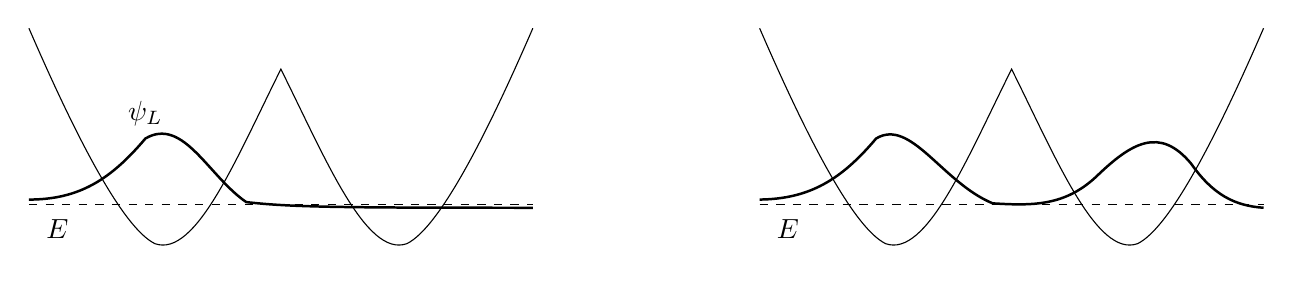
\begin{tikzpicture}[x=0.8cm,y=0.8cm]
\begin{scope}[shift={(-5.8,0)}]
\draw (-4,2.7) .. controls (-3.35,1.2) and (-2.55,-0.45) .. (-2.0,-0.72)
      .. controls (-1.35,-0.95) and (-0.7,0.65) .. (0,2.05)
      .. controls (0.7,0.65) and (1.35,-0.95) .. (2.0,-0.72)
      .. controls (2.55,-0.45) and (3.35,1.2) .. (4,2.7);
\draw[dashed] (-4,-0.10) -- (4,-0.10);
\node at (-3.55,-0.48) {$E$};
\draw[line width=0.9pt] (-4,-0.02) .. controls (-3.2,-0.02) and (-2.7,0.30) .. (-2.15,0.95)
      .. controls (-1.55,1.30) and (-1.15,0.35) .. (-0.55,-0.06)
      .. controls (0.15,-0.14) and (0.9,-0.15) .. (4,-0.15);
\node at (-2.15,1.35) {$\psi_L$};
\end{scope}
\begin{scope}[shift={(5.8,0)}]
\draw (-4,2.7) .. controls (-3.35,1.2) and (-2.55,-0.45) .. (-2.0,-0.72)
      .. controls (-1.35,-0.95) and (-0.7,0.65) .. (0,2.05)
      .. controls (0.7,0.65) and (1.35,-0.95) .. (2.0,-0.72)
      .. controls (2.55,-0.45) and (3.35,1.2) .. (4,2.7);
\draw[dashed] (-4,-0.10) -- (4,-0.10);
\node at (-3.55,-0.48) {$E$};
\draw[line width=0.9pt] (-4,-0.02) .. controls (-3.2,-0.01) and (-2.7,0.30) .. (-2.15,0.95)
      .. controls (-1.6,1.28) and (-1.1,0.25) .. (-0.30,-0.08)
      .. controls (0.35,-0.12) and (0.85,-0.12) .. (1.35,0.35)
      .. controls (1.9,0.88) and (2.35,1.15) .. (2.85,0.55)
      .. controls (3.2,0.05) and (3.55,-0.12) .. (4,-0.15);
\end{scope}
\end{tikzpicture}
\end{adjustbox}
\caption{Eine saubere Neuzeichnung der ersten Skizzen an der Tafel. Links ist der einseitige Probezustand \(\psi_L\) zu sehen, bei dem man so tut, als sei die Barriere effektiv unendlich hoch. Rechts wurde dieselbe Wellenfunktion symmetrisch durch die Barriere hindurch fortgesetzt. Das veranschaulicht das geringe, aber von null verschiedene Eindringen, aus dem schließlich der echte gerade Grundzustand hervorgeht.}
\end{figure}

Quantenmechanisch ist die Barriere jedoch nicht wirklich unendlich hoch. Die Wellenfunktion im Barrierenbereich ist nicht exakt null, sondern nur sehr klein. Dieses winzige Eindringen ist entscheidend. Es macht aus der Näherung mit linker und rechter Mulde ein echtes Mischungsproblem.

\section{Paritätseigenzustände und exponentielle Aufspaltung der Energieniveaus}

Die Vorstellung lokalisierter Zustände wird nun durch einen Satz unterbrochen: Ist das Potential symmetrisch, dann lassen sich die exakten Energieeigenfunktionen so wählen, dass sie bei Spiegelung entweder symmetrisch oder antisymmetrisch sind.

\begin{theorem}
Gilt \(V(x)=V(-x)\) in einer Dimension, so können die Eigenfunktionen des Hamiltonoperators so gewählt werden, dass sie entweder
\[
\psi(x)=\psi(-x)
\qquad \text{or} \qquad
\psi(x)=-\psi(-x).
\]
\end{theorem}

Nun folgt die Korrektur. Die einseitigen Zustände \(\psi_L\) und \(\psi_R\) sind weder symmetrisch noch antisymmetrisch und können daher keine exakten Eigenzustände des vollständigen Hamiltonoperators sein. Bei hoher Barriere sind sie lediglich gute Näherungszustände. Die wahren Eigenzustände sind die symmetrischen und antisymmetrischen Linearkombinationen:
\begin{align}
\psi_+ &= \frac{\psi_L+\psi_R}{\sqrt{2}},\\
\psi_- &= \frac{\psi_L-\psi_R}{\sqrt{2}}.
\end{align}
Mit der Notation, die an der Tafel stehen bleibt, bezeichnen wir ihre Energien als
\begin{align}
H\psi_+ &= (E_1-\epsilon)\psi_+,\\
H\psi_- &= (E_1+\epsilon)\psi_-.
\end{align}
Die gesamte Aufspaltung beträgt somit
\begin{equation}
\Delta E = (E_1+\epsilon)-(E_1-\epsilon)=2\epsilon .
\end{equation}

\begin{figure}[htbp]
\centering
\includegraphics[width=0.92\linewidth]{lecture_08_frame_02.png}
\caption{Die symmetrisch durch das Doppelmuldenpotential fortgesetzte Wellenfunktion. Unter der Barriere ist ihre Amplitude klein, aber von null verschieden; darin liegt der Ursprung der Aufspaltung der Energieniveaus.}
\lectureframe{00:06:19}
\end{figure}

\begin{figure}
\centering
\begin{tikzpicture}[x=1cm,y=1cm]
\draw[->] (0,0) -- (0,3);
\node[left] at (0,2.8) {energy};
\draw (-0.35,1.60) -- (0.35,1.60);
\node[left] at (-0.45,1.60) {$\psi_L,\psi_R$};
\node at (1.7,1.60) {$\Longrightarrow$};
\draw (3.0,1.32) -- (3.75,1.32);
\draw (3.0,1.88) -- (3.75,1.88);
\draw[dashed] (2.8,1.60) -- (3.95,1.60);
\node[right] at (3.9,1.32) {$\psi_+,\ E_1-\epsilon$};
\node[right] at (3.9,1.88) {$\psi_-,\ E_1+\epsilon$};
\node[below] at (3.37,1.60) {$E_1$};
\end{tikzpicture}
\caption{Die Herleitung der Tunnelaufspaltung an der Tafel. Die näherungsweisen Zustände links und rechts sind nahezu entartet, doch die exakten symmetrischen und antisymmetrischen Eigenzustände sind um einen kleinen Betrag \(2\epsilon\) aufgespalten.}
\end{figure}

Die Reihenfolge der Energieniveaus macht die physikalische Aussage deutlich. Der symmetrische Zustand hat eine geringfügig niedrigere Energie, weil seine Wellenfunktion im Barrierenbereich glatter verläuft. Wenn sie in die Barriere eindringt und sich symmetrisch fortsetzt, sinkt die Energie um einen winzigen Betrag. Der antisymmetrische Zustand hat eine geringfügig höhere Energie, weil der erste angeregte Zustand in einer Dimension einen Knoten besitzt und dieser in diesem symmetrischen Problem in der Mitte liegt. Zusätzliche Krümmung kostet kinetische Energie.

Der Effekt ist sehr klein, exponentiell klein mit zunehmender Breite und Höhe der Barriere. Eine explizite WKB-Formel brauchen wir hier nicht; entscheidend ist, dass die Aufspaltung real, aber winzig ist. Außerdem gilt: Das globale Vorzeichen einer Wellenfunktion hat keine physikalische Bedeutung. Ersetzt man \(\psi_-\) durch \(-\psi_-\), ändert sich der Zustand nicht.

\section{Zeitentwicklung und Oszillation zwischen links und rechts}

Stellen wir nun die dynamische Frage: Was geschieht, wenn wir ein Teilchen in die linke Mulde setzen? Das ist der entscheidende Schritt, denn die Oszillation ist die zeitabhängige Erscheinungsform desselben Mischungsphänomens.

Die inversen Beziehungen lauten
\begin{align}
\psi_L &= \frac{\psi_+ + \psi_-}{\sqrt{2}},\\
\psi_R &= \frac{\psi_+ - \psi_-}{\sqrt{2}}.
\end{align}
Ein anfangs links lokalisierter Zustand ist also
\begin{equation}
\psi(0)=\psi_L=\frac{\psi_+ + \psi_-}{\sqrt{2}}.
\end{equation}
Er ist kein Energieeigenzustand und muss sich daher nichttrivial entwickeln.

Wir verwenden die übliche Schr\"odingerKonvention\(e^{-iEt}\). Eine gemeinsame Phase hat keine beobachtbaren Auswirkungen; nur die relative Phase zwischen den beiden Energiekomponenten kann die Wahrscheinlichkeit von einer Mulde in die andere verlagern.

Mit dieser Konvention gilt
\begin{equation}
\psi(t)=\frac{1}{\sqrt{2}}\left(e^{-i(E_1-\epsilon)t}\psi_+ + e^{-i(E_1+\epsilon)t}\psi_-\right).
\end{equation}
Dies ist die bereinigte Fassung der Formel von der Tafel. Wir klammern nun die gemeinsame Phase aus:
\begin{equation}
\psi(t)=\frac{e^{-iE_1 t}}{\sqrt{2}}\left(e^{i\epsilon t}\psi_+ + e^{-i\epsilon t}\psi_-\right).
\end{equation}
Eine Phase läuft nun in der einen Richtung um den Einheitskreis, die andere in der entgegengesetzten. Der Zustand ändert sich nur, weil diese beiden Phasen auseinanderlaufen.

Um die Oszillation zwischen links und rechts explizit zu sehen, setzen wir die Definitionen von \(\psi_\pm\) ein:
\begin{align}
\psi(t)
&= \frac{e^{-iE_1 t}}{2}
\left[e^{i\epsilon t}(\psi_L+\psi_R)+e^{-i\epsilon t}(\psi_L-\psi_R)\right] \\
&= \frac{e^{-iE_1 t}}{2}
\left[(e^{i\epsilon t}+e^{-i\epsilon t})\psi_L+(e^{i\epsilon t}-e^{-i\epsilon t})\psi_R\right] \\
&= e^{-iE_1 t}\left[\psi_L\cos(\epsilon t)+i\,\psi_R\sin(\epsilon t)\right].
\end{align}
Dies ist die zentrale Herleitung des Kapitels. In der Zweizustandsnäherung, wobei \(\psi_L\) und \(\psi_R\) orthonormal sind, lauten die Wahrscheinlichkeiten
\begin{equation}
P_L(t)=\cos^2(\epsilon t),
\qquad
P_R(t)=\sin^2(\epsilon t).
\end{equation}
Das System oszilliert also. Zu Zwischenzeiten befindet es sich tatsächlich in einer Überlagerung; zum Beispiel sind die Wahrscheinlichkeiten auf beiden Seiten gleich, wenn \(\epsilon t=\pi/4\). Die Phasen entwickeln sich kontinuierlich, und mit ihnen ändert sich die Lokalisierung kontinuierlich.

Die Herleitung an der Tafel bestimmt den ersten Zeitpunkt, zu dem sich das relative Vorzeichen umkehrt. Gesucht ist der Zeitpunkt, für den
\begin{equation}
e^{-i\epsilon t}=-\,e^{i\epsilon t},
\end{equation}
gilt. Dies ist der an der Tafel sichtbare entscheidende Schritt. Multiplikation beider Seiten ergibt
\begin{equation}
e^{2i\epsilon t}=-1.
\end{equation}
Für das erste Auftreten gilt
\begin{equation}
2\epsilon t=\pi,
\qquad\text{so}\qquad
t_{L\to R}=\frac{\pi}{2\epsilon}.
\end{equation}

\begin{figure}[htbp]
\centering
\includegraphics[width=0.94\linewidth]{lecture_08_frame_05.png}
\caption{Die Berechnung der relativen Phase an der Tafel. Bei \(e^{2i\epsilon t}=-1\) werden die beiden Energiekomponenten gegenphasig; damit ergibt sich die erste Übergangszeit \(2\epsilon t=\pi\). In der gesetzten Herleitung wird eine einheitliche Schr\"odinger-Phasenkonvention verwendet.}
\lectureframe{00:17:52}
\end{figure}
Zu diesem Zeitpunkt gilt
\begin{equation}
\psi(t_{L\to R}) \propto \frac{\psi_+-\psi_-}{\sqrt{2}}=\psi_R.
\end{equation}
Die globale Phase ist unerheblich. Entscheidend ist, dass sich das anfangs links platzierte Teilchen zum rechts lokalisierten Zustand entwickelt hat. Nach einem weiteren gleich langen Zeitintervall schwingt es wieder zurück. Mischung und Oszillation gehören zusammen.

Die Gleichung ist eindeutig: Ein kleines \(\epsilon\) bedeutet langsame Oszillation und eine lange Übergangszeit. Keiner der lokalisierten Zustände hat eine bestimmte Energie, aber die beiden exakten Energiekomponenten erhalten die Energie und entwickeln sich genau so, wie es sein soll.

\section{Analogien zu Neutrinos, Ammoniak und Spin}

Das Doppelmuldenpotential liefert ein Muster für unsere ursprüngliche Frage zu Neutrinos. Ein Neutrino, das zusammen mit einem Elektron erzeugt wird, heißt Elektron-Neutrino; eines, das zusammen mit einem Myon erzeugt wird, heißt Myon-Neutrino. Diese Flavorbezeichnungen beschreiben die Erzeugungs- und Nachweiskanäle. Die Zustände mit bestimmten Massen und damit bestimmten Energien freier Teilchen bei festem Impuls bilden eine andere Basis.

In der einfachsten, maximal gemischten Zweizustandsnäherung gilt
\begin{equation}
|\nu_e\rangle \sim \frac{|m_1\rangle+|m_2\rangle}{\sqrt{2}},
\qquad
|\nu_\mu\rangle \sim \frac{|m_1\rangle-|m_2\rangle}{\sqrt{2}},
\end{equation}
wobei die Masseneigenzustände die Rolle von \(\psi_+\) und \(\psi_-\) und die Flavorzustände die Rolle von \(\psi_L\) und \(\psi_R\) spielen. Bei realen Neutrinomischungen steht anstelle dieser gleichen Koeffizienten eine nichttriviale Mischungsmatrix; der Mechanismus wird hier aber bereits sichtbar.

Ein Elektron-Neutrino wird in einem Prozess mit Beteiligung eines Elektrons erzeugt, so wie man ein Teilchen in die linke Mulde setzen kann. Während eines kurzen Fluges haben seine beiden Massenkomponenten nahezu dieselbe Phase angesammelt, sodass eine Wechselwirkung es weiterhin als Elektron-Flavor identifiziert. Über eine große Flugstrecke laufen ihre Phasen auseinander. Eine spätere geladene Stromwechselwirkung kann dann ein Myon statt eines Elektrons erzeugen: Der Zustand hat einen Myon-Flavoranteil erhalten. Wiederholt man das Experiment bei unterschiedlichen Entfernungen oder Energien, zeigt sich die Oszillation.

Es gibt keinen Widerspruch zur Energieerhaltung. Die Masse-Energie-Eigenzustände verhalten sich genau so, wie es Eigenzustände tun sollen. Es ist die Flavorüberlagerung, die sich entwickelt. Im relativistischen Grenzfall wird die beobachtbare relative Phase durch Massendifferenzen zum Quadrat bestimmt, schematisch
\begin{equation}
\Delta\phi_{ij}\simeq \frac{\Delta m_{ij}^{,2}L}{2E}.
\end{equation}
Die Oszillation zeigt daher, dass nicht alle Neutrinomassen identisch sein können; mindestens zwei Masseneigenzustände unterscheiden sich in ihrer Masse.

\begin{classroomqa}
\lecturetimestamp{00:24:06}
\audiencequestion{Wodurch wird die kleine Aufspaltung \(\epsilon\) im Doppelmuldenbeispiel bestimmt?}
\lecturerresponse{Sie hängt von der Teilchenmasse sowie von Höhe und Breite der Barriere ab. Tunneln reagiert exponentiell empfindlich auf diese Größen, sodass eine mäßige Änderung der Barriere eine große relative Änderung von \(\epsilon\) bewirken kann.}
\end{classroomqa}

\begin{classroomqa}
\lecturetimestamp{00:24:26}
\audiencequestion{Wurde dieses Oszillationsphänomen tatsächlich beobachtet?}
\lecturerresponse{Ja. Tunnelaufspaltungen werden in gewöhnlichen Quantensystemen beobachtet, und Flavoroszillationen werden bei Neutrinos beobachtet. Die Mechanismen unterscheiden sich im mikroskopischen Detail, doch beide verwirklichen dieselbe Phasenentwicklung in einem Zweizustandssystem.}
\end{classroomqa}

\begin{classroomqa}
\lecturetimestamp{00:24:34}
\audiencequestion{Wie hängt die Neutrinooszillation mit der Neutrinomasse zusammen?}
\lecturerresponse{Die propagierenden Eigenzustände haben unterschiedliche Massen und sammeln daher unterschiedliche Phasen an. Ihre Interferenz verändert die Flavorzusammensetzung. In einer realistischen relativistischen Beschreibung bestimmen die Massendifferenzen zum Quadrat die Oszillation, nicht eine wörtlich zeitabhängige Masse eines einzelnen Teilchens.}
\end{classroomqa}

\begin{classroomqa}
\lecturetimestamp{00:25:02}
\audiencequestion{Ist die Neutrinomasse lediglich vorherrschende Theorie oder eine experimentelle Tatsache?}
\lecturerresponse{Die Oszillation ist eine experimentelle Tatsache und erfordert von null verschiedene Massendifferenzen. Die absolute Massenskala ist eine separate und schwierigere Messgröße, doch das Minimalbild, in dem alle Neutrinos masselos sind, ist experimentell ausgeschlossen.}
\end{classroomqa}

\subsection{Ammoniakinversion: eine echte Barriere}

Ein Ammoniakmolekül \(\mathrm{NH}_3\) hat eine trigonal-pyramidale Struktur: Die drei Wasserstoffatome liegen in einer Ebene, und das Stickstoffatom befindet sich auf einer Seite dieser Ebene. Es gibt eine gleichwertige Konfiguration, bei der das Stickstoffatom auf der anderen Seite liegt. Die beiden lokalisierten Konfigurationen sind keine exakten stationären Zustände. Das Stickstoffatom kann durch die Wasserstoffebene tunneln, wodurch symmetrische und antisymmetrische Energieeigenzustände sowie eine kleine Inversionsaufspaltung entstehen. Dies ist der physikalische Ursprung derselben Mathematik im Ammoniakmaser.

\begin{classroomqa}
\lecturetimestamp{00:25:11}
\audiencequestion{Ist in Ammoniak die Konfiguration, in der das Stickstoffatom durch die Wasserstoffebene tritt, die Barriere?}
\lecturerresponse{Ja. Die Molekülenergie ist in beiden pyramidenförmigen Konfigurationen minimal, während die ebene Konfiguration eine höhere Energie hat. Das Tunneln durch diese Konfiguration koppelt die beiden Seiten.}
\end{classroomqa}

\begin{classroomqa}
\lecturetimestamp{00:27:10}
\audiencequestion{Was entspricht der physikalischen Barriere zwischen Elektron- und Myon-Neutrinos?}
\lecturerresponse{Es gibt keine echte räumliche Barriere. Die Analogie ist algebraischer Art: Eine außerdiagonale Kopplung im Neutrino-Hamiltonoperator mischt die Flavorbasis. Bei Ammoniak entsteht diese Kopplung durch Tunneln; bei Neutrinos ist sie Teil der Masse- und Mischungsstruktur.}
\end{classroomqa}

\subsection{Spinpräzession: Mischung ohne Tunneln}

Dieselbe Algebra ist uns bereits beim Spin begegnet. Betrachten wir die beiden Zustände \(|\uparrow_z\rangle\) und \(|\downarrow_z\rangle\). Ohne Magnetfeld sind sie entartet. Nun schalten wir ein Magnetfeld in \(x\)-Richtung ein. Die Energieeigenzustände sind dann nicht mehr die \(z\)-Eigenzustände, sondern die \(x\)-polarisierten Zustände. Mit den vorläufigen Bezeichnungen links--rechts von der Tafel gilt
\begin{align}
|L_x\rangle &= \frac{|\uparrow_z\rangle+|\downarrow_z\rangle}{\sqrt{2}},\\
|R_x\rangle &= \frac{|\uparrow_z\rangle-|\downarrow_z\rangle}{\sqrt{2}}.
\end{align}
Diese Zustände sind direkte Analogien zu \(\psi_+\) und \(\psi_-\). Das am Feld ausgerichtete beziehungsweise entgegengesetzt ausgerichtete magnetische Moment hat eine geringfügig andere Energie. Sind diese Energien \(E\mp\epsilon\), so entwickelt sich ein anfangs nach oben gerichteter Spin wie folgt:
\begin{equation}
|\uparrow_z,t\rangle
= e^{-iEt}\left[\cos(\epsilon t)\,|\uparrow_z\rangle
+ i\sin(\epsilon t)\,|\downarrow_z\rangle\right].
\end{equation}
Dies ist dieselbe Formel wie beim Doppelmuldenpotential; hier handelt es sich jedoch um eine kontinuierliche Spinpräzession um die \(x\)-Achse. Ausgehend von \(+z\) durchläuft der Spin transversale Richtungen, erreicht nach einer halben Präzessionsperiode \(-z\) und kehrt nach einer weiteren halben Periode zurück. Eine Messung von \(S_z\) ergibt weiterhin nur oben oder unten; der sich kontinuierlich ändernde Spin-Zustand bestimmt die Wahrscheinlichkeiten dafür. Der Mechanismus erfordert kein Tunneln. Er erfordert lediglich, dass der Hamiltonoperator in einer anderen Basis diagonal ist als in der Präparationsbasis.

\begin{classroomqa}
\lecturetimestamp{00:32:25}
\audiencequestion{Was geschieht in diesem Bild mit dem Tau-Neutrino?}
\lecturerresponse{Es mischt sich ebenfalls. Das reale Problem umfasst drei Flavorzustände und drei Massenzustände, sodass eine dreidimensionale Mischungsmatrix die Zweizustandsrotation ersetzt. Das Prinzip der Phaseninterferenz bleibt unverändert.}
\end{classroomqa}

\begin{classroomqa}
\lecturetimestamp{00:32:57}
\audiencequestion{Zeigt der Spin unmittelbar nach Anlegen des transversalen Feldes noch nach oben, und kann er auf uns zu oder von uns weg zeigen?}
\lecturerresponse{Nach sehr kurzer Zeit zeigt er mit hoher Wahrscheinlichkeit noch nach oben; die Wahrscheinlichkeit für einen Spin nach unten ist klein. Der Zustand präzediert kontinuierlich um die Feldachse und durchläuft die transversalen Richtungen \(\pm y\). Wenn er anfangs senkrecht zum Feld stand, bleibt er senkrecht zum in \(x\)-Richtung weisenden Feld. Eine Messung entlang einer beliebigen gewählten Achse ergibt weiterhin einen der diskreten Eigenwerte dieser Achse.}
\end{classroomqa}

\begin{classroomqa}
\lecturetimestamp{00:34:30}
\audiencequestion{Wird ein schwaches Feld gewählt, damit der Spin nie in Richtung des Feldes zeigt?}
\lecturerresponse{Nein. Die Geometrie ergibt sich aus der Präzession um die Feldachse, nicht aus der Schwäche des Feldes. Ein schwaches Feld macht lediglich die Energieaufspaltung und die Präzessionsfrequenz klein, sodass eine langsame Oszillation entsteht, ähnlich wie beim Neutrinobeispiel.}
\end{classroomqa}

Die Stärke der Neutrinomischung und die kleinen Neutrinomassen sind Parameter, deren tieferen Ursprung das ursprüngliche minimale Standardmodell nicht erklärt. Die Neutrinomasse weist daher über dieses Minimalmodell hinaus, auch wenn die beobachtete Skala sehr klein ist und möglicherweise auf Physik bei einer weit entfernten Energieskala zurückgeht.

\begin{classroomqa}
\lecturetimestamp{00:36:27}
\audiencequestion{Ist die Oszillation der Grund dafür, dass wir wissen, dass Neutrinos Masse haben?}
\lecturerresponse{Sie ist der entscheidende direkte Beleg dafür, dass die propagierenden Komponenten unterschiedliche Massen haben. Wären alle relevanten Komponenten exakt masselos und entartet, würden sie keine massenabhängige relative Phase ansammeln, und eine Vakuum-Flavoroszillation dieser Art träte nicht auf.}
\end{classroomqa}

\begin{classroomqa}
\lecturetimestamp{00:37:57}
\audiencequestion{Sollte sich ein Neutrino nach einer halben Periode halb wie ein Elektron-Flavor und halb wie ein Myon-Flavor verhalten?}
\lecturerresponse{Im idealen symmetrischen Zweizustandsmodell treten gleiche Wahrscheinlichkeiten bei einem Viertel der vollständigen Wahrscheinlichkeitsperiode auf, während die vollständige Umwandlung beim ersten Maximum eintritt. Bei realen Drei-Flavor-Oszillationen sind die Mischungswinkel verschieden, es gibt mehrere Frequenzen sowie Einschränkungen durch den Spin-Helizitätszustand und Materieeffekte; eine vollständige symmetrische Umwandlung ist daher nicht allgemein zu erwarten.}
\end{classroomqa}

\begin{classroomqa}
\lecturetimestamp{00:38:36}
\audiencequestion{Muss sich die Geschwindigkeit eines solaren Neutrinos ändern, um den Impuls zu erhalten, wenn sich die Massenkomponenten unterscheiden?}
\lecturerresponse{Ein Flavorzustand ist eine kohärente Überlagerung von Komponenten mit festen Massen; seine Masse ist keine klassische, mit der Zeit oszillierende Größe. In der üblichen Beschreibung mit gleichem Impuls haben die Komponenten geringfügig unterschiedliche Energien und Gruppengeschwindigkeiten, während sie in einer Beschreibung mit gleicher Energie geringfügig unterschiedliche Impulse haben. Bei konsistenter Behandlung liefern beide Konventionen dieselbe beobachtbare Oszillationsphase.}
\end{classroomqa}

Diese Phasenentwicklung löste das alte Defizit der solaren Neutrinos. Frühe Detektoren waren vorwiegend für Elektron-Neutrinos empfindlich. Neutrinos, die die Sonne als Elektron-Flavor verließen, konnten daher teilweise als Myon- oder Tau-Flavor ankommen und dem betreffenden Nachweiskanal entgehen. Die detaillierte Berechnung für die Sonne berücksichtigt Drei-Flavor-Mischungen und Materieeffekte; die grundlegende Einsicht zeigt sich jedoch bereits im Doppelmuldenpotential: Präparation und Ausbreitung verwenden unterschiedliche Basen.

\section{Exkurs: elektrisches Dipolmoment, Symmetrie und die Behauptung einer ``kugelförmigen'' Elektron}

Da wir ohnehin schon über Teilchenphänomenologie sprechen, machen wir eine Pause von der formalen Mathematik. Ein populärwissenschaftlicher Artikel beschrieb eine neue Schranke für das elektrische Dipolmoment des Elektrons mit der Behauptung, das Elektron sei als Kugel nachgewiesen worden. Diese zugespitzte Aussage vermengt drei verschiedene Fragen: Was misst ein elektrisches Dipolmoment? Was bedeutet Rotationssymmetrie für einen Quantenzustand? Und welche Größe hat das Experiment tatsächlich eingeschränkt?

\subsection{Was wurde gemessen?}

Gemessen beziehungsweise eingeschränkt wurde das elektrische Dipolmoment des Elektrons. Für räumlich getrennte Ladungen \(\pm q\) ist das Dipolmoment
\begin{equation}
\mathbf d = q\,\boldsymbol{\ell},
\end{equation}
wobei \(\boldsymbol{\ell}\) der Abstandsvektor ist. Ein von null verschiedenes Dipolmoment bedeutet, dass die Ladungsverteilung gegenüber einem Bezugspunkt verschoben ist.

Beim Elektron lautet die entscheidende Frage jedoch nicht bloß, ob die Ladung in irgendeiner beliebigen Richtung außermittig liegt. Das Elektron besitzt Spin und damit eine Achse. Es hat außerdem ein magnetisches Moment. Die physikalisch sinnvolle Frage ist, ob die Ladungsverschiebung mit dieser Achse zusammenhängt:
\begin{equation}
\mathbf d_e \parallel \boldsymbol{\mu}_e
\qquad \text{or equivalently} \qquad
\mathbf d_e \parallel \mathbf S .
\end{equation}
Dieser Zusammenhang ist es, der mit dem elektrischen Dipolmoment des Elektrons gemeint ist. Begrifflich fragt man, ob ein elektrisches Feld die beiden Spinorientierungen eines spinpolarisierten Elektrons energetisch aufspaltet:
\begin{equation}
H_{\mathrm{EDM}}=-\mathbf d_e\cdot \mathbf E,
\qquad
\mathbf d_e=d_e\frac{\mathbf S}{|\mathbf S|}.
\end{equation}
Das tatsächliche Tischversuchsexperiment ist deutlich subtiler als ein freies Elektron zwischen Kondensatorplatten, doch es nutzt genau diese Idee von Symmetrie und Energieverschiebung.

\subsection{Warum ein verschwindendes elektrisches Dipolmoment keine Kugelform bedeutet}

Die erste Korrektur ist einfach: Ein Körper kann kein Dipolmoment besitzen und trotzdem keine Kugel sein. Ein zentriertes Ellipsoid hat auf beiden Seiten gleich viel Ladung und somit kein Dipolmoment, kann aber ein Quadrupolmoment haben. Eine noch komplexere Verteilung kann weder ein Dipol- noch ein Quadrupolmoment aufweisen und trotzdem ein höheres Multipolmoment besitzen. Die Messung eines Multipolkoeffizienten bestimmt nicht die gesamte Form.

In der Quantenmechanik ist das Wort ``Form'' schwieriger zu fassen. Stellen wir uns ein hantelförmiges Molekül aus zwei Atomen mit annähernd fester Bindungslänge vor. Vernachlässigen wir radiale Schwingungen und betrachten nur Rotationen. Die Rotationszustände werden durch den Drehimpuls bezeichnet. Ist das Molekül bosonisch, so gilt für den niedrigsten Rotationszustand \(J=0\). Da der Drehimpuls Rotationen erzeugt,
\begin{equation}
\begin{gathered}
J=0 \quad\Longrightarrow\\
\text{rotationally invariant ground state.}
\end{gathered}
\end{equation}
ist der Quantenzustand rotationsinvariant, obwohl jedes Bild mit bestimmter Orientierung wie eine Hantel aussieht. Man kann ihn als kohärente Überlagerung aller Orientierungen beschreiben. Den Zustand als ``kugelförmig'' zu bezeichnen, ist für manche Messungen nützlich und für andere irreführend.

Machen wir eine Momentaufnahme. Eine Momentaufnahme entspricht einer Messung der Orientierung; eine hinreichend präzise Orientierungsbestimmung versetzt das System in einen im Winkel lokalisierten Zustand. Ein solcher Zustand kann nicht zugleich einen bestimmten Drehimpuls haben. Dies ist die Rotationsversion der Orts--Impuls-Unschärferelation: Eine Lokalisierung des Winkels führt notwendigerweise zu einer Streuung der Drehimpulse und damit zu Rotationsanregungen.

Für einen starren Rotator gilt
\begin{equation}
E_J=\frac{J(J+1)}{2I},
\end{equation}
sodass die zur Auflösung nötige Energie durch das Trägheitsmoment \(I\) bestimmt wird. Eine Hantel in einer Sporthalle hat ein sehr großes \(I\) und extrem dicht benachbarte Rotationsniveaus; gewöhnliches Licht kann sie leicht so stark stören, dass eine Orientierung erkennbar wird. Bei einem Molekül ist der Niveauabstand größer. Bei einem kompakten Hadron ist er noch viel größer. Reicht die Energie der Sonde nicht aus, um die erste auflösbare Rotationsstruktur anzuregen, zeigen wiederholte Messungen nur den rotationsgemittelten Grundzustand.

Ein Meson lässt sich grob als Zweiteilchensystem aus Quark--Antiquark auffassen. Seine ersten orbitalen Anregungen kosten Hunderte Millionen Elektronenvolt oder mehr und liegen damit weit oberhalb der Energie optischer Photonen. Eine Sonde niedriger Energie kann daher keine Momentaufnahme der zugrunde liegenden Orientierung machen. Ob etwas ``kugelförmig oder nicht'' ist, hängt teilweise davon ab, welcher Zustand präpariert wird, und teilweise von der Auflösung des Messgeräts.

Am Elektron wird die Frage noch präziser. Es ist ein Teilchen mit Spin \(\tfrac12\) und kein Rotationsskalar. Ein spinpolarisierter Zustand besitzt eine Achse und ein magnetisches Moment. Das vertraute Bild umlaufender Ladung um diese Achse ist lediglich ein anschauliches Hilfsbild---ein punktförmiges Dirac-Teilchen ist keine buchstäblich rotierende kleine Kugel---; es erinnert uns jedoch richtigerweise daran, dass sich das magnetische Moment mit dem Spin umkehrt. Die Frage nach dem elektrischen Dipolmoment lautet, ob die elektrische Ladungsverschiebung mit derselben Achse zusammenhängt. Ein Nullbefund macht das Elektron nicht zu einer klassischen Kugel.

\begin{classroomqa}
\lecturetimestamp{00:57:30}
\audiencequestion{Würde eine Verschiebung eines Teils der Elektronenladung die Ladungsquantisierung verletzen?}
\lecturerresponse{Nein. Die Ladungsquantisierung legt die Gesamtladung fest. Ein Dipolmoment betrifft das erste räumliche Moment der Ladungsverteilung oder gleichbedeutend eine zulässige Kopplung eines Punktteilchens an das elektrische Feld; es erfordert keine Änderung der Gesamtladung um einen Bruchteil.}
\end{classroomqa}

\begin{classroomqa}
\lecturetimestamp{00:58:00}
\audiencequestion{Sind elektrische Dipolmomente durch die Quantenfeldtheorie verboten?}
\lecturerresponse{Nicht durch die Quantenfeldtheorie an sich. Sie sind verboten, wenn bestimmte diskrete Symmetrien exakt gelten. Werden diese Symmetrien verletzt, ist ein Operator für das elektrische Dipolmoment zulässig, auch wenn sein Koeffizient äußerst klein sein kann.}
\end{classroomqa}

\subsection{Parität und Zeitumkehr}

Der eigentliche Inhalt der Diskussion um das elektrische Dipolmoment ist die Symmetrie. Unter Parität verhält sich ein elektrisches Dipolmoment wie ein gewöhnlicher polarer Vektor, während sich ein magnetisches Moment wie ein axialer Vektor verhält:
\begin{align}
P:\qquad &\mathbf d_e \to -\mathbf d_e,
&\boldsymbol{\mu}_e \to \boldsymbol{\mu}_e .
\end{align}
Unter Zeitumkehr kehrt sich der Kreisstrom, der das magnetische Moment definiert, um; eine statische elektrische Ladungsverschiebung dagegen nicht:
\begin{align}
T:\qquad &\mathbf d_e \to \mathbf d_e,
&\boldsymbol{\mu}_e \to -\boldsymbol{\mu}_e .
\end{align}
Daher ist ein von null verschiedenes, an der Spinachse des Elektrons ausgerichtetes elektrisches Dipolmoment sowohl bei exakter Paritätssymmetrie als auch bei exakter Zeitumkehrsymmetrie verboten:
\begin{equation}
(P\ \text{exact}) \Rightarrow \mathbf d_e=0,
\qquad
(T\ \text{exact}) \Rightarrow \mathbf d_e=0.
\end{equation}

Die Geometrie lohnt es sich, genauer zu betrachten. Ein magnetisches Moment entsteht durch einen stromartigen Kreisstrom. Eine Spiegelung kehrt gewöhnliche polare Vektoren um, lässt aber den axialen Vektor normal zu dieser Schleife unverändert. Eine Ladungsverschiebung entlang der Achse kehrt sich dagegen um. Ein Elektron, bei dem \(\mathbf d_e\) parallel zu \(\boldsymbol\mu_e\) ist, würde durch Spiegelung daher in eines mit gleicher magnetischer Orientierung, aber umgekehrter Beziehung zwischen elektrischem und magnetischem Moment überführt. Wäre die Parität exakt erhalten und gäbe es nur eine Elektronensorte, müssten die beiden Beschreibungen dasselbe Teilchen darstellen; nur \(d_e=0\) ist damit vereinbar.

Die Zeitumkehr führt auf andere Weise zum selben Schluss. Beim Rückwärtslaufen des Films kehrt sich der Strom und damit \(\boldsymbol\mu_e\) um, eine statische Ladungsverschiebung wird jedoch nicht umgekehrt. Ein Zustand mit parallelen Momenten geht in einen mit antiparallelen Momenten über. Exakte Zeitumkehrsymmetrie würde wiederum \(d_e=0\) erfordern.

\begin{figure}[htbp]\centering
\begin{tikzpicture}[>=Stealth,scale=0.95]
  \node[font=\bfseries] at (1.0,2.25) {original};
  \draw[->,very thick,blue!70!black] (0.65,0) -- (0.65,1.65);
  \draw[->,very thick,red!75!black] (1.35,0) -- (1.35,1.65);
  \node[blue!70!black,below] at (0.65,0) {$\boldsymbol\mu$};
  \node[red!75!black,below] at (1.35,0) {$\mathbf d$};

  \node[font=\bfseries] at (4.5,2.25) {parity};
  \draw[->,very thick,blue!70!black] (4.15,0) -- (4.15,1.65);
  \draw[->,very thick,red!75!black] (4.85,1.65) -- (4.85,0);
  \node[blue!70!black,below] at (4.15,0) {$\boldsymbol\mu$};
  \node[red!75!black,below] at (4.85,0) {$-\mathbf d$};

  \node[font=\bfseries] at (8.0,2.25) {time reversal};
  \draw[->,very thick,blue!70!black] (7.65,1.65) -- (7.65,0);
  \draw[->,very thick,red!75!black] (8.35,0) -- (8.35,1.65);
  \node[blue!70!black,below] at (7.65,0) {$-\boldsymbol\mu$};
  \node[red!75!black,below] at (8.35,0) {$\mathbf d$};
\end{tikzpicture}\caption{Der aus der Tafelargumentation rekonstruierte Symmetrietest. Die Parität kehrt das elektrische Dipolmoment um, nicht aber das axiale magnetische Moment; die Zeitumkehr kehrt das magnetische Moment um, nicht aber die statische elektrische Ladungsverschiebung. Jede der beiden exakten Symmetrien verbietet ein permanentes elektrisches Dipolmoment parallel zum Spin.}\end{figure}

\begin{figure}[htbp]\centering
\includegraphics[width=0.94\linewidth]{lecture_08_frame_06.png}\caption{Die Skizzen der magnetischen Achse und der Ladungsverschiebung während der Argumentation zur Zeitumkehr. Das kompakte TikZ-Diagramm oben hebt den Transformationsinhalt von der teilweise weggewischten Tafelzeichnung aus der Vorlesung ab.}\lectureframe{01:06:10}\end{figure}

\begin{classroomqa}\lecturetimestamp{01:06:38}\audiencequestion{Kehren sich bei der Zeitumkehr sowohl Ströme als auch Ladungen um?}\lecturerresponse{Ströme kehren sich um, weil sich die Geschwindigkeiten umkehren; die elektrische Ladung selbst tut das nicht. Die Ladungskonjugation \(C\), nicht die Zeitumkehr \(T\), kehrt das Vorzeichen der Ladung um.}\end{classroomqa}

\begin{classroomqa}\lecturetimestamp{01:07:01}\audiencequestion{Bedeutet der antiunitäre Charakter der Zeitumkehr, dass die nichtrelativistische Quantenmechanik nicht zeitumkehrinvariant ist?}\lecturerresponse{Nein. Gerade durch Antiunitarität lässt sich die Zeitumkehr in der Quantenmechanik konsistent darstellen: Sie komplex konjugiert Amplituden und kehrt Impulse und Spins um. Ob ein bestimmter Hamiltonoperator invariant ist, ist eine davon getrennte Frage.}\end{classroomqa}

\begin{classroomqa}\lecturetimestamp{01:07:19}\audiencequestion{Muss man für die Diskussion eines elektrischen Dipolmoments annehmen, dass das Elektron ein endliches Volumen hat und nicht punktförmig ist?}\lecturerresponse{Nein. Ein effektiver Hamiltonoperator für ein Punktteilchen kann \(-d_e\,\widehat{\mathbf S}\!\cdot\!\mathbf E\) enthalten. Im Experiment wird untersucht, ob entgegengesetzte Spinorientierungen in einem elektrischen Feld unterschiedliche Energien haben; eine buchstäblich ausgedehnte Ladungswolke muss dabei nicht aufgelöst werden.}\end{classroomqa}

Die schwache Wechselwirkung ist nicht paritätssymmetrisch; die Parität ist in ihren chiralen Kopplungen maximal verletzt. Auch die Zeitumkehr ist keine exakte Symmetrie, doch die bekannte Verletzung im Standardmodell trägt nur auf außerordentlich niedrigem Niveau zum elektrischen Dipolmoment des Elektrons bei. Man kann einen von null verschiedenen Beitrag des Standardmodells berechnen, doch er liegt weit unterhalb der hier erörterten Empfindlichkeit. Ein Nullresultat ist daher mit dem Standardmodell vereinbar, schränkt aber Erweiterungen---etwa die Supersymmetrie und andere neue Wechselwirkungen---ein, die eine deutlich stärkere Zeitumkehrverletzung hervorrufen können.

Der grundlegende Gedanke des Experiments ist einfach. Ein Magnetfeld weist ein magnetisches Dipolmoment nach, indem es die Spinorientierungen energetisch aufspaltet. Ein elektrisches Feld würde ein elektrisches Dipolmoment durch eine zusätzliche, mit dem Spin korrelierte Energieverschiebung nachweisen. Tatsächliche Präzisionsexperimente verwenden Atome oder Moleküle, lange Kohärenzzeiten der Präzession, Umkehrungen der angelegten Felder und eine sorgfältige Kontrolle systematischer Effekte, statt ein isoliertes Elektron in einem naiven Versuchsaufbau zu untersuchen.

\begin{classroomqa}\lecturetimestamp{01:11:02}\audiencequestion{War die Suche nach dem elektrischen Dipolmoment ein Hochenergiekollisionsexperiment oder ein Experiment mit materiellen Objekten?}\lecturerresponse{Es handelte sich um ein Präzisionsexperiment im Labormaßstab: Elektronen waren in einer kontrollierten atomaren oder molekularen Umgebung gebunden und elektrischen sowie magnetischen Feldern ausgesetzt. Die Energie ist niedrig, doch die Empfindlichkeit für winzige symmetrieverletzende Verschiebungen erlaubt es, indirekt neue Physik bei hohen Energien zu untersuchen.}\end{classroomqa}

\begin{classroomqa}\lecturetimestamp{01:12:21}\audiencequestion{Schränkt das Nullresultat ein, welche Änderungen des Standardmodells noch möglich sind?}\lecturerresponse{Ja, grundsätzlich: Jedes Modell sagt einen Koeffizienten voraus und belegt damit einen bestimmten Parameterbereich. Für die detaillierte numerische Ausschlussgrenze ist eine spezialisierte Berechnung erforderlich, aber die allgemeine Logik ist eindeutig---Eine präzisere Übereinstimmung mit dem Standardmodell lässt weniger Spielraum für Alternativen, die ein großes elektrisches Dipolmoment vorhersagen.}\end{classroomqa}

\begin{classroomqa}\lecturetimestamp{01:13:09}\audiencequestion{Ist Zeitumkehrsymmetrie eine Voraussetzung für die Erhaltung von Quanteninformation?}\lecturerresponse{Nein. Eine unitäre Zeitentwicklung erhält die Information auch dann, wenn ein Hamiltonoperator unter \(T\) nicht invariant ist. Ein Teilchen in einem fest vorgegebenen Magnetfeld ist ein vertrautes Beispiel: In zeitumgekehrt betrachteten Filmen wählt das Feld eine Orientierung aus, sofern man nicht auch das Feld umkehrt; dennoch bleibt die Quantenentwicklung unitär. Unter den üblichen Annahmen einer lokalen Lorentz-invarianten Quantenfeldtheorie ist die kombinierte Transformation \(CPT\) eine Symmetrie; die Unitarität wird dadurch jedoch nicht gewährleistet.}\end{classroomqa}

Die Pause kann nun enden. Die Nullmessung besagt, dass beim Elektron bis zur angegebenen Empfindlichkeitsgrenze kein elektrisches Dipolmoment nachgewiesen wurde. Sie besagt weder, dass das Elektron eine Kugel ist, noch stellt sie das Standardmodell infrage; sie erschwert es, manche vorgeschlagenen Abweichungen von diesem Modell aufrechtzuerhalten.

\section{Rückkehr zur zweiten Quantisierung: Fouriertransformationen, Impulsmoden und Lokalität}

Wir hatten uns mit der zweiten Quantisierung beschäftigt. Beginnen wir noch einmal in Ruhe mit einer vertrauten Tatsache über gewöhnliche Wellenfunktionen eines einzelnen Teilchens und übertragen sie dann auf Operatoren. Der Zusammenhang mit Fouriertransformationen ist exakt und einfach.

\subsection{Vom Ortsraum zum Impulsraum}

Das kleine \(\psi\), nicht das große \(\Psi\), ist die Wellenfunktion eines einzelnen Teilchens. Im Ortsraum ist
\begin{equation}
P(x)=|\psi(x)|^2
\end{equation}
die Wahrscheinlichkeitsdichte, das Teilchen am Ort \(x\) zu finden. Die Wellenfunktion im Impulsraum ist ihre Fouriertransformierte:
\begin{equation}
\tilde{\psi}(p)=\int dx\,\psi(x)\,\frac{e^{-ipx}}{\sqrt{2\pi}},
\end{equation}
Die inverse Beziehung lautet
\begin{equation}
\psi(x)=\int dp\,\tilde{\psi}(p)\,\frac{e^{ipx}}{\sqrt{2\pi}}.
\end{equation}
Damit ist
\begin{equation}
P(p)=|\tilde{\psi}(p)|^2
\end{equation}
die Wahrscheinlichkeitsdichte für den Impuls \(p\).

Wir verwenden \(\hbar=1\). Die beiden Transformationen sind invers zueinander: Kennt man eine der Wellenfunktionen, lässt sich die andere bestimmen; ihre Betragsquadrate beantworten jedoch unterschiedliche Messfragen.

Für ein freies Teilchen gilt
\begin{equation}
H=\frac{p^2}{2m},
\end{equation}
Impuls-Eigenzustände sind also zugleich Energie-Eigenzustände, und ihre Wellenfunktionen im Ortsraum sind ebene Wellen:
\begin{equation}
\psi_p(x)\propto e^{ipx}.
\end{equation}
Davon geht die Formulierung in zweiter Quantisierung aus.

\begin{figure}[htbp]\centering
\includegraphics[width=0.94\linewidth]{lecture_08_frame_07.png}\caption{Das Fourierpaar aus Orts--- und Impulsraum für die Wellenfunktion eines einzelnen Teilchens. Die Unterscheidung zwischen dem kleinen \(\psi\) und dem im Folgenden eingeführten Feldoperator mit großem griechischem Buchstaben ist wesentlich.}\lectureframe{01:20:00}\end{figure}

\subsection{Feldoperatoren im Orts- und Impulsraum}

Kehren wir nun zum Feldoperator zurück. An der Tafel werden seine Vernichtungs- und Erzeugungsanteile als \(\Psi_-(x)\) und \(\Psi_+(x)\) geschrieben. Behalten wir diese Schreibweise zunächst bei:
\begin{align}
\Psi_-(x) &= \sum_i a_i\,\psi_i(x),\\
\Psi_+(x) &= \sum_i a_i^\dagger\,\psi_i^*(x).
\end{align}
Dabei ist \(\psi_i(x)\) die gewöhnliche Einteilchen-Wellenfunktion der \(i\)-ten Mode, während \(a_i\) und \(a_i^\dagger\) Teilchen in dieser Mode vernichten beziehungsweise erzeugen. Von hier an ist es zweckmäßig, die Bezeichnungen umzubenennen:
\[
\Psi(x)\equiv \Psi_-(x),
\qquad
\Psi^\dagger(x)\equiv \Psi_+(x).
\]

Für ein freies Teilchen wird das diskrete Modenlabel \(i\) durch das kontinuierliche Impulslabel \(p\) ersetzt. Mit den ebenen Wellen \(e^{ipx}\) erhält man die bekannten rekonstruierten Formeln:
\begin{align}
\Psi(x) &= \int \frac{dp}{\sqrt{2\pi}}\,a(p)\,e^{ipx},\\
\Psi^\dagger(x) &= \int \frac{dp}{\sqrt{2\pi}}\,a^\dagger(p)\,e^{-ipx}.
\end{align}
Sie sind die Analoga der gewöhnlichen Fouriertransformation für Feldoperatoren. Wie zuvor lassen sie sich exakt invertieren:
\begin{align}
a(p) &= \int \frac{dx}{\sqrt{2\pi}}\,\Psi(x)\,e^{-ipx},\\
a^\dagger(p) &= \int \frac{dx}{\sqrt{2\pi}}\,\Psi^\dagger(x)\,e^{ipx}.
\end{align}
Die Faktoren \(1/\sqrt{2\pi}\) sind eine Konvention, durch die Vorwärts- und Rücktransformation dieselbe Normierung erhalten.

Der begriffliche Gehalt ist einfach. \(\Psi^\dagger(x)\) erzeugt ein Teilchen am Ort \(x\), während \(a^\dagger(p)\) ein Teilchen mit Impuls \(p\) erzeugt. Die Erzeugungsoperatoren im Orts- und Impulsraum sind Fourier-konjugiert, ebenso wie \(\psi(x)\) und \(\tilde{\psi}(p)\) in der gewöhnlichen Quantenmechanik Fourier-konjugiert sind.

Ist kein Teilchen mit Impuls \(p\) vorhanden, vernichtet \(a(p)\) den Zustand. Sind Teilchen mit diesem Impuls vorhanden, entfernt der Operator eines davon mit dem üblichen Besetzungszahlkoeffizienten. Entsprechend entfernt \(\Psi(x)\) ein Teilchen am Ort \(x\), wobei dies im distributionellen Sinn oder nach Verschmierung zu einem Wellenpaket zu verstehen ist. Für jede Teilchensorte braucht man einen eigenen Feldoperator; ein Feld kann nicht jede Art von Teilchen erzeugen.

\subsection{Bosonische Kommutatoren und die Unabhängigkeit räumlich getrennter Messungen}

Die nächste Tatsache lässt sich direkt aus den Definitionen herleiten. Für Bosonen gilt
\begin{equation}
[a_i,a_j^\dagger]=\delta_{ij},
\qquad
[a_i,a_j]=0,
\qquad
[a_i^\dagger,a_j^\dagger]=0.
\end{equation}
Im Kontinuum lautet die entsprechende Beziehung
\begin{equation}
[a(p),a^\dagger(p')]=\delta(p-p').
\end{equation}
Berechnen wir nun den Feldkommutator bei gleichen Zeiten mithilfe der diskreten Entwicklung:
\begin{align}
[\Psi(x),\Psi^\dagger(y)]
&= \sum_{i,j}\psi_i(x)\psi_j^*(y)\,[a_i,a_j^\dagger] \\
&= \sum_i \psi_i(x)\psi_i^*(y) \\
&= \delta(x-y),
\end{align}
wobei im letzten Schritt die Vollständigkeit der Einteilchenbasis verwendet wird. Entsprechend gilt
\begin{equation}
[\Psi(x),\Psi(y)]=0,
\qquad
[\Psi^\dagger(x),\Psi^\dagger(y)]=0.
\end{equation}

\begin{figure}[htbp]\centering
\includegraphics[width=0.94\linewidth]{lecture_08_frame_08.png}\caption{Der Modenkommutator und sein Gegenstück im Ortsraum an der Tafel. Aus der Vollständigkeit folgt, dass \(\delta_{ij}\) zur räumlichen Delta-Distribution \(\delta(x-y)\) wird.}\lectureframe{01:31:00}\end{figure}

Entscheidend ist nicht bloß, dass \(\Psi\) nicht hermitesch ist. Definieren wir hermitesche Quadraturen:
\begin{equation}
Q(x)=\frac{\Psi(x)+\Psi^\dagger(x)}{\sqrt{2}},
\qquad
P(x)=\frac{\Psi(x)-\Psi^\dagger(x)}{i\sqrt{2}}.
\end{equation}
Ihr Kommutator am selben Ort enthält ebenfalls die Delta-Distribution. Die beiden lokalen Quadraturen sind daher in demselben Sinn konjugiert wie Ort und Impuls. Eine präzisere Bestimmung der einen vergrößert die Unbestimmtheit der anderen.

\begin{classroomqa}\lecturetimestamp{01:32:03}\audiencequestion{Was bedeutet die Deltafunktion für \(x=y\)}? Ist der Kommutator überall groß?\lecturerresponse{Die Deltafunktion ist eine Distribution und keine gewöhnliche Funktion mit einem endlichen Funktionswert an einem Punkt. Für getrennte Argumente verschwindet sie und liefert nur dann ein endliches Ergebnis, wenn man sie gegen eine Testfunktion integriert. Verschmiert man die Felder über einen Detektorbereich endlicher Ausdehnung, wird die formale Singularität am selben Ort zum üblichen endlichen kanonischen Kommutator zweier Moden.}\end{classroomqa}

Für \(x\neq y\) verschwindet dagegen der Kommutator bei gleichen Zeiten. Operationen, die in zwei disjunkten Bereichen lokalisiert sind, können unabhängig voneinander ausgeführt werden: Eine Messung des Feldes hier versetzt das Feld dort nicht in einen quantenmechanischen Stoß. Dies ist die nichtrelativistische Vorstufe der relativistischen Mikrokausalität bei gleichen Zeiten. In einer relativistischen Theorie kommutieren physikalische lokale Observablen bei raumartig getrennten Ereignissen, zwischen denen kein Lichtsignal vermitteln kann.

Der Gegensatz zu nichtkommutierenden Observablen ist vertraut. Wegen \([x,p]=i\) stört eine präzise Ortsmessung den Impuls, und ein präziser Impulszustand ist räumlich ausgedehnt. Da verschiedene Spin-Komponenten nicht miteinander kommutieren, macht eine scharfe Präparation einer Komponente eine andere unbestimmt. Ein von null verschiedener Kommutator zwischen räumlich getrennten lokalen Observablen würde entsprechend bedeuten, dass eine Operation in einem Bereich den anderen beeinflusst, im Widerspruch zur geforderten kausalen Unabhängigkeit.

\begin{classroomqa}\lecturetimestamp{01:37:51}\audiencequestion{Zeigen EPR- und Verschränkungsexperimente, dass eine Messung hier eine entfernte Messung beeinflusst?}\lecturerresponse{Sie zeigen Korrelationen, keinen kontrollierbaren kausalen Einfluss. Verschränkte Messergebnisse verletzen die klassische Faktorisierung, doch die lokalen Statistiken am entfernten Detektor lassen sich nicht dadurch ändern, dass man hier eine Messung auswählt oder durchführt. Die Kommutativität raumartig getrennter Observablen ist die operatorielle Aussage, die dieser Unabhängigkeit ohne Signalübertragung zugrunde liegt.}\end{classroomqa}

Beim nächsten Mal ändert sich die Algebra. Erzeugungs- und Vernichtungsoperatoren für Fermionen erfüllen Antikommutationsrelationen. Bei naiver Betrachtung kommutieren Fermionenfelder an getrennten Punkten nicht; die Felder selbst lassen sich daher nicht als unmittelbar messbare bosonische Observablen deuten. Physikalische fermionische Observablen sind gerade Kombinationen---Dichten, Ströme, Spannungstensoren---, und für diese lokalen Observablen gilt wieder die erforderliche Kommutativität bei raumartiger Trennung. Damit beginnt die Behandlung der zweiten Quantisierung für Fermionen.
